\section{Design}
\label{sec:design}
We now discuss the design philosophy behind sybilhunter, our Sybil detection
tool.  Sybilhunter takes as input archived Tor network data, and then attempts
to isolate Sybil groups.  The big picture is shown in Figure~\ref{fig:system}.
We motivate our design decisions with the experience we gained by manually
analyzing numerous Sybil groups in the Tor network.  We iteratively improved
and refactored sybilhunter when we experienced operational shortcomings.  We
further augment our design with ideas from related work, e.g., Cao et al.
observed that Sybil groups have things in common and changes happen more or
less at the same time~\cite{Cao2014a}.

\begin{figure}[t]
	\centering
	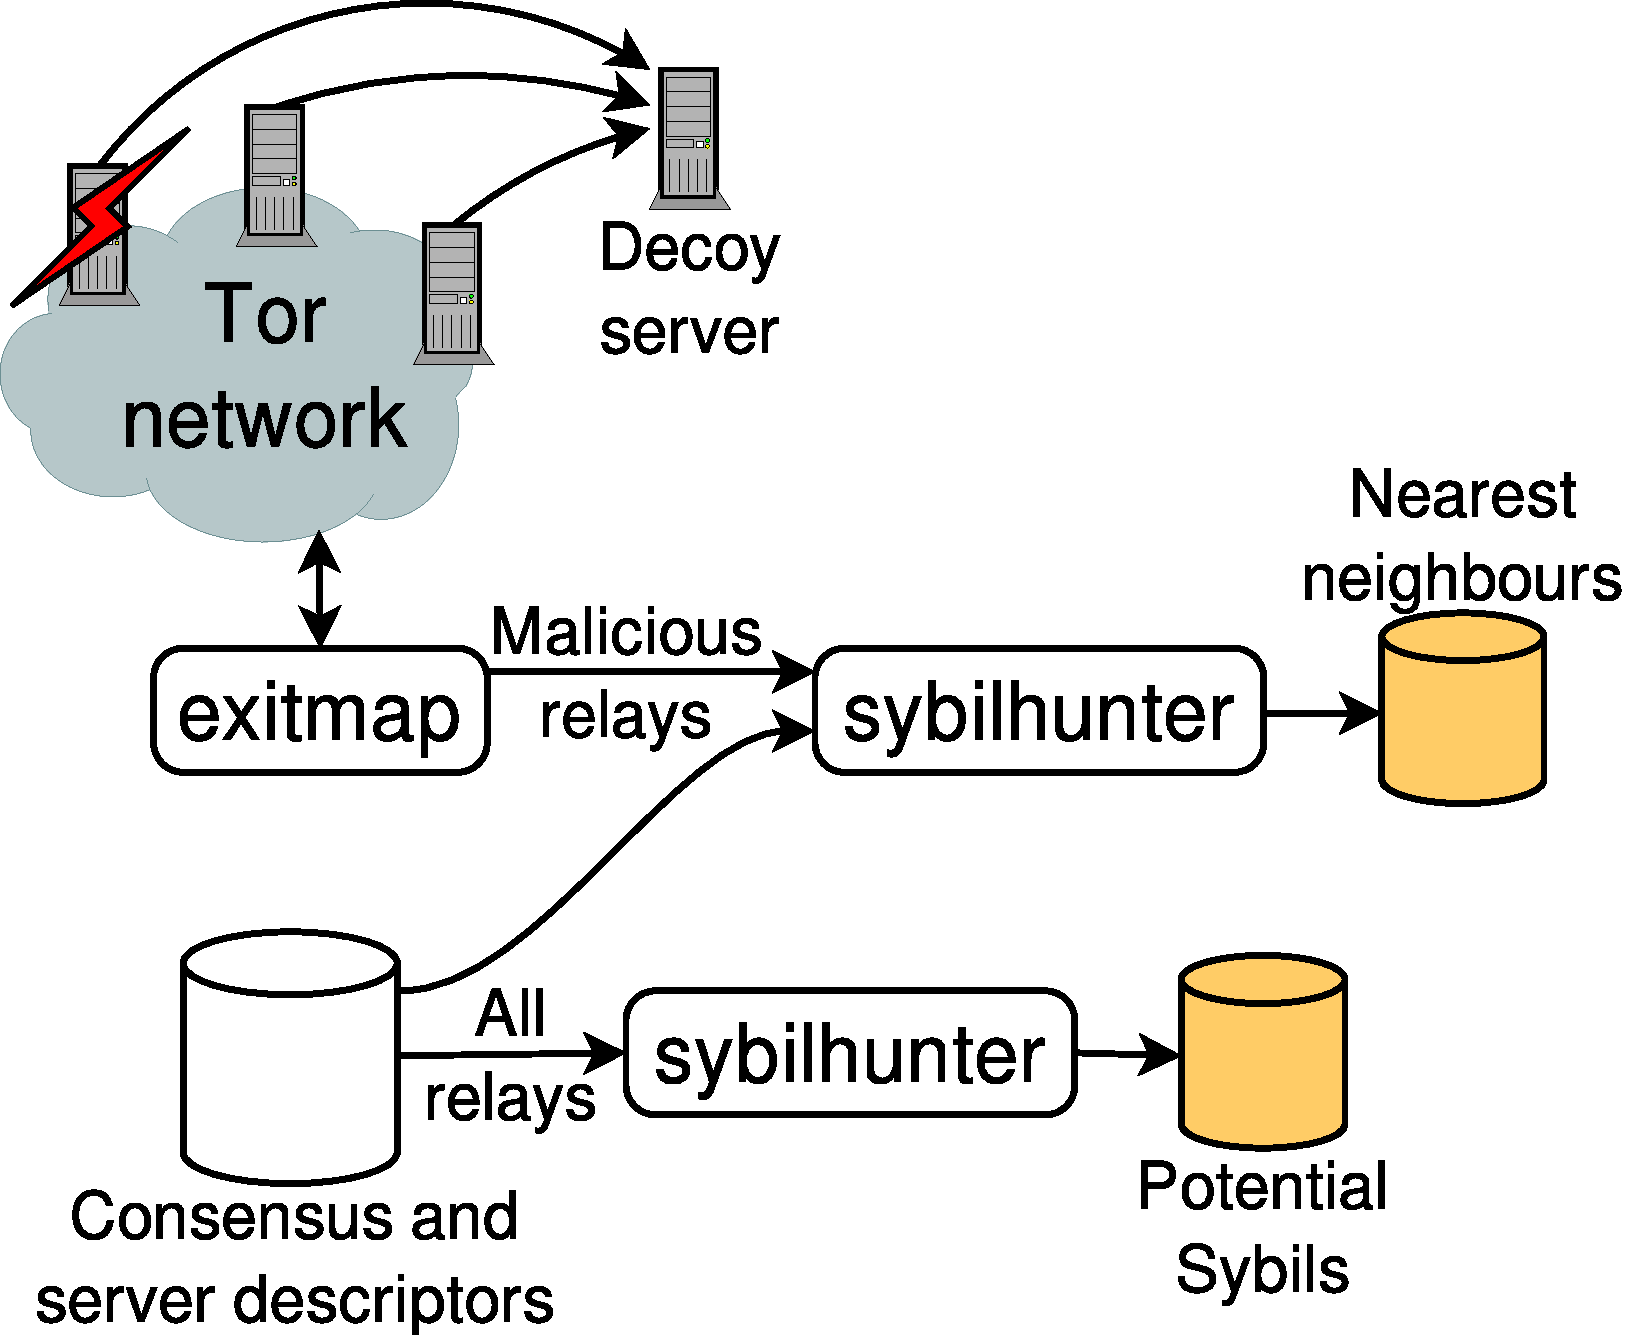
\includegraphics[width=0.42\textwidth]{diagrams/system_architecture.pdf}
	\caption{Our system architecture.  Two different data sets serve as input
		to sybilhunter, our Sybil detection tool; 1) archived consensuses and
		server descriptors, and 2) malicious relays that we gather by running
		exitmap~\cite{Winter2014a}.  Sybilhunter then attempts to extract Sybil
		groups from the given data.}
	\label{fig:system}
\end{figure}

Sybilhunter is designed to run in different scenarios.  We can 1) run it over
historical network data, ranging back to 2007, 2) run it online to detect new
Sybils as they join the network, and 3) use it to find relays that are
potentially associated with previously discovered bad exit relays.

Generally speaking, we seek to isolate relays that are similar in
\emph{appearance} (\S~\ref{sec:nearest-neighbor}) as well as in \emph{behavior}
(\S~\ref{sec:churn-time-series}, \S~\ref{sec:uptime-matrix}, and
\S~\ref{sec:fingerprint-analysis}).  The following sections discuss our data sets
and analysis modules of sybilhunter.

\mynote{Can we model the arrival rate of relay descriptor as Poisson process
and find outliers in it?}

\subsection{Data sets}
\label{sec:datasets}
We employ two types of data sets, both of which are illustrated in
Figure~\ref{fig:system}.  First, we mine \emph{archived consensuses and server
descriptors} for relay clusters and second, we use the \emph{output of the
exitmap scanner} (in combination with archived data) to find associated,
malicious relays.

\subsubsection{Consensuses and router descriptors}
We took the data sets we use for our analyses from CollecTor~\cite{collector},
a service run by The Tor Project that archives network data such as
consensuses, router descriptors, and network status votes.  Some of the
archived data dates back to as early as 2004, allowing us to restore arbitrary
Tor network states in the last ten years.  CollecTor archives numerous data
sources, but not all are relevant for our hunt for Sybils, which is why we only
analyse the following two:

\begin{description}
	\item[Descriptors] Tor relays and bridges periodically upload server
		descriptors, which capture their configuration, to directory
		authorities.  Relays upload their descriptors no later than every 18
		hours, or sooner, depending on certain conditions.

	\item[Consensuses] The Tor network's consensus contains a list of all
		running Tor relays.  Directory authorities vote hourly on the state of
		the network, and the outcome is the consensus.  Every relay status in
		the consensus contains a digest that is used to obtain the relay's
		respective descriptor, as can be seen in Figure~\ref{fig:datasets}.
\end{description}

\begin{figure}[t]
	\centering
	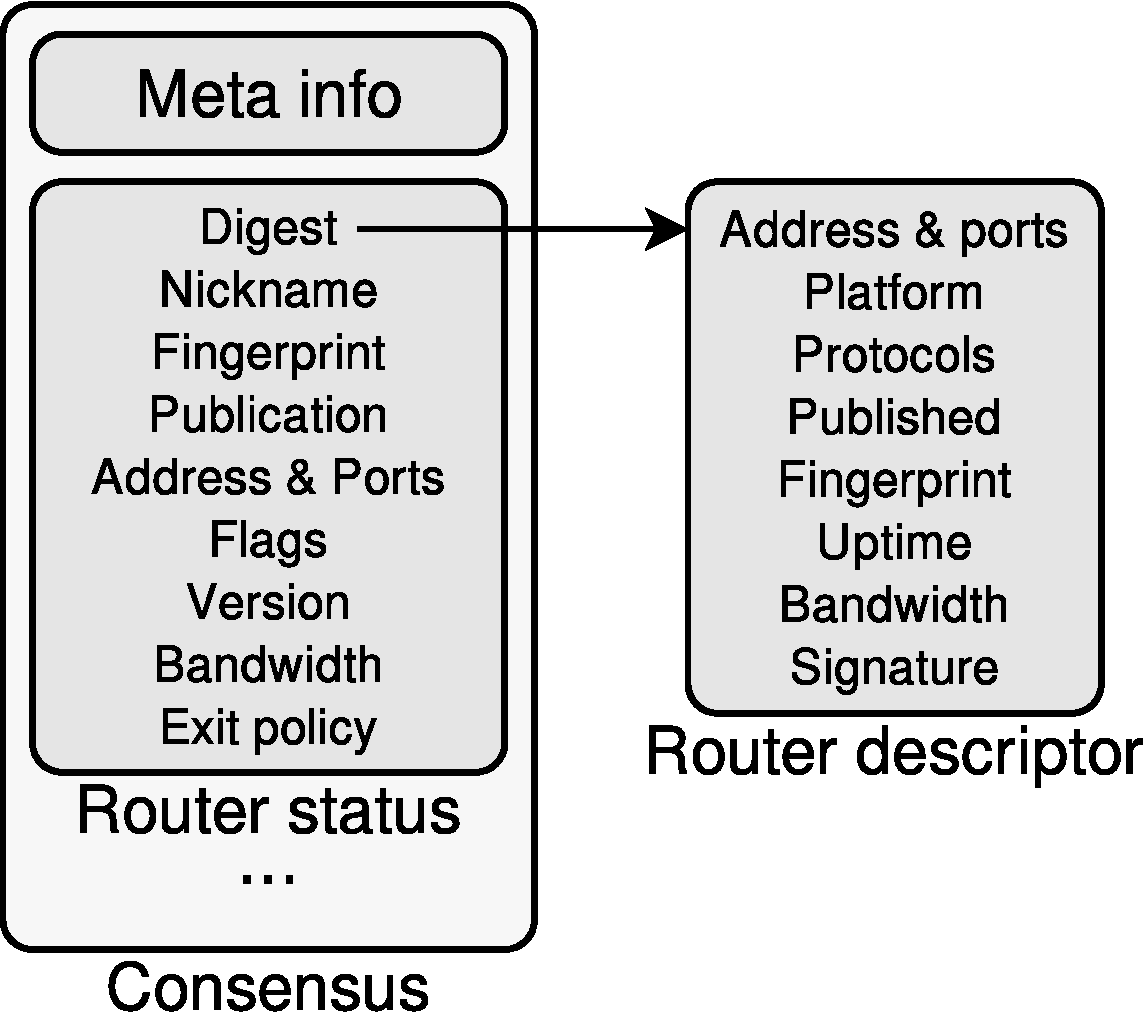
\includegraphics[width=0.3\textwidth]{diagrams/data_sets.pdf}
	\caption{Our data set contains consensuses and router descriptors.  This
		diagram shows how they relate to each other.}
	\label{fig:datasets}
\end{figure}

Table~\ref{tab:collector-dataset} gives an overview of the size of our data
sets.  We found it challenging to process such large amounts of data.  We
started by using the Python parsing library Stem, which is maintained by The Tor
Project.  The size of the data sets as well as the amount of files turned out to
be difficult to handle for Stem because it was implemented in an interpreted,
dynamic language.

\begin{table}[t]
\centering
\begin{tabular}{l c c c}
\textbf{Data set} & \textbf{Files} & \textbf{Size} & \textbf{Time span} \\
\hline
% 47677982862 bytes.
Consensuses & 67,671 & 44 GiB & 10/2007 -- 07/2015 \\
% 48252370463 bytes.
Descriptors & 30,759,243 & 44 GiB & 12/2005 -- 07/2015 \\
% 1375933490 bytes.
% Torperf data & 18,348 & 1 GiB & 07/2009 -- 07/2015 \\
\end{tabular}
\caption{Characterization of our data sets.}
\label{tab:collector-dataset}
\end{table}

\begin{table}[t]
\centering
\begin{tabular}{l c p{4cm}}
\textbf{Discovery} & \textbf{\# of relays} & \textbf{Incident} \\
\hline
% Message-ID: <20150926174033.GB27610@nymity.ch>
2015-09-26 & 6 & Blocking STARTTLS over SMTP. \\
% Message-ID: <20150804202838.GA4774@nymity.ch>
2015-08-04 & 4 & Onion service impersonation by rewriting onion domains. \\
% Message-ID: <20150630022923.GA2340@nymity.ch>
2015-06-29 & 55 & Onion service impersonation by rewriting onion domains. \\
% Message-ID: <20150423004031.GA11395@nymity.ch>
2015-04-22 & 70 & Onion service impersonation by rewriting onion domains. \\
% Message-ID: <20150311125831.GD23215@nymity.ch>
2015-03-11 & 1 & Injected iframe into relayed HTML. \\
\end{tabular}
\caption{Characterization of the bad exit relays we collected.}
\label{tab:exitmap-dataset}
\end{table}

We then implemented a new parser from scratch in the Go programming
language~\cite{zoossh}.  Our parser consists of approximately 2,000 lines of
code (and 1,000 more lines for tests) and supports strict and lazy parsing, to
minimize unnecessary parsing.  According to our benchmarks, our parser is able
to parse approximately 27 consensuses per second.\footnote{Measured on an Intel
Core i7 2.9 GHz CPU.  We placed our data sets on a solid state drive to
minimize I/O.}  Stem, for comparison, averages at around 1.8 consensuses per
second.\footnote{Note, however, that Stem parses slightly more fields than our
parser, which means that both parsers would be closer together in a fair
comparison.}

Figure~\ref{fig:datasets} illustrates the relationship between our data.
Primarily, we are interested in the hourly consensus files.  A consensus file
consists of \emph{router statuses} that contain basic information about Tor
relays such as its bandwidth, flags, and exit policy.  As of August 2015,
consensuses contain approximately 6,000 router statuses.  Every router status
contains a digest that is used to locate its corresponding \emph{router
descriptor}.  It is important to understand that router descriptors are
published as they were received by Tor relays whereas consensus files are voted
on, and published, by directory authorities.  Some fields in a router status
are also subject to verification.  For example, the Tor network operates
bandwidth scanners that verify if a relay is able to sustain the bandwidth it
claims to handle in its router descriptor.

\subsubsection{Malicious relays}
We use a second, complementary data set that consists of malicious exit relays
we gather by running exitmap~\cite[\S 3.1]{Winter2014a}.  The dataset is shown
in Table~\ref{tab:exitmap-dataset}.  Exitmap is a Python-based scanning
framework for Tor exit relays.  Exitmap modules perform a network task that can
then be run over all exit relays.  One use case is HTTPS MitM detection: A
module can fetch the X.509 certificate of a web server over all exit relays and
then compare the fingerprint to the expected, valid fingerprint.  In addition to
the original modules, exitmap's authors shared with us, we implemented modules
to detect HTML tampering and TLS downgrading.  Our modules ran from August 2014
to August 2015 and discovered 225 malicious exit relays, which we all reported
to The Tor Project.
% blockchain.info tampering
% <20140811014615.GB23748@nymity.ch> 1
% <20140920132357.GC8751@nymity.ch> 1
% <20141021133016.GA11247@nymity.ch> 2
% <20141025182433.GA23244@nymity.ch> 1
% <20150109195428.GA29115@nymity.ch> 23
% <20150210154109.GD10777@nymity.ch> 1
% <20150804202838.GA4774@nymity.ch> 4
% <20150630022923.GA2340@nymity.ch> 55
% <20150605120807.GA20320@nymity.ch> 49
% <20150423004031.GA11395@nymity.ch> 70
% <20150311131506.GE23215@nymity.ch> 18

We include malicious exit relays in our data set because we found that they
frequently \emph{surface in groups}, i.e., an attacker runs the same attack on
several, physically distinct exit relays.  Winter et al.'s work~\cite[\S
5.2]{Winter2014a} showed that attackers make an effort to stay under the radar,
which is why we cannot only rely on active probing to find and block such
relays.  We also seek to find the \emph{nearest neighbors} of each newly
discovered malicious relay, which we discuss in
Section~\ref{sec:nearest-neighbor}.

\subsection{Threat model}
\label{sec:threat_model}
\mynote{Threat model is vague.  Ideas for better phrasing?}

Sybilhunter, our Sybil detection tool, can process \emph{past data} just as
\emph{future data}.  Future data, however, can be manipulated by adversaries
that seek to evade our system and the powerful nature of Sybil
attacks~\cite{Douceur2002a} limits us in what we can defend against.  This is
reflected in our adversarial assumptions, which we now discuss.  We expect that
an an adversary \emph{does}:
\begin{itemize}
	\item Run multiple Tor relays.

	\item Add Tor relays all at once or slowly over time.

	\item Run active or passive attacks.

	\item Make a limited effort to stay under the radar by diversifying
		different aspects of their Tor relays.
\end{itemize}

We expect that an adversary \emph{does not}:
\begin{itemize}
	\item Have infinite resources to create undetectable Sybils.
\end{itemize}


\mynote{The order of subsections here isn't fixed yet.  There might be a better
way of organizing them.}

\subsection{Network churn time series}
\label{sec:churn-time-series}
The churn rate of a distributed system is the rate of joining and leaving
network participants---relays in the Tor network.  An unexpectedly high churn
rate between two subsequent consensuses can reveal Sybils because Sybil
operators frequently start and stop their Sybils at the same time for convenient
administration.

The Tor Project is maintaining a Python script~\cite{doctor} that determines the
number of relay fingerprints in new consensuses that have never been seen
before.  If that number exceeds the static threshold 49, an email alert is sent.
We reimplemented the script in sybilhunter and ran it over all archived
consensus documents, dating back to 2007.  The script raised 47 alerts in nine
years, all of which seemed true positives, i.e., they should be of interest to
directory authority operators.  The script did not raise false positives because
the median number of new fingerprints in a consensus is only six---significantly
below the conservative threshold of 49.  The script's conservative threshold
probably causes false negatives, but we cannot determine the rate because we
lack ground truth.  In addition, The Tor Project's script can be defeated by a
``trickling'' attack in which Sybils are slowly added over time.  We now extend
The Tor Project's approach to make it more robust against these shortcomings.

We found that churn anomalies worthy of our attention range from \emph{flat
hills} (see Figure~\ref{fig:flat-hill}) to \emph{sudden spikes} (see
Figure~\ref{fig:sudden-spike}).  The former can be a sign of an event that
affected a large number of relays in the network\footnote{This happened shortly
after the heartbleed vulnerability.  The Tor Project advised relay operators
to generate new keys.  Naturally, relay operators did not do this at the same
hour, but gradually over approximately two days.} while the latter can happen if
an attacker adds several dozen relays in one or two hours.

\begin{figure}[t]
	\centering
	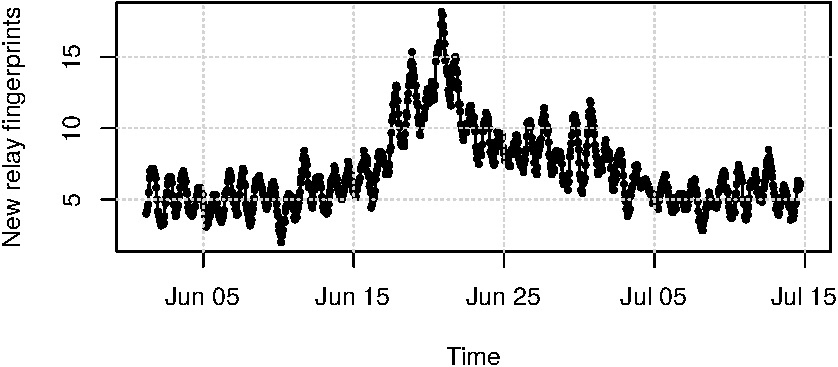
\includegraphics[width=0.47\textwidth]{diagrams/flat-hill.pdf}
	\caption{Flat hill in 2009.  Smoothed using moving average with a window
	size of 12.}
	\label{fig:flat-hill}
\end{figure}

\begin{figure}[t]
	\centering
	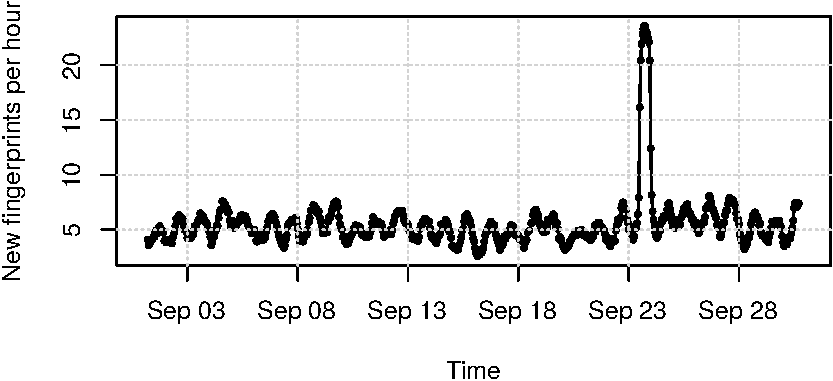
\includegraphics[width=0.47\textwidth]{diagrams/sudden-spike.pdf}
	\caption{Sudden spike in 2010.  Smoothed using moving average with a window
	size of 12.}
	\label{fig:sudden-spike}
\end{figure}

To quantify the churn rate $\sigma$ between two subsequent consensus documents,
we adapt the formula proposed by Godfrey et al.~\cite{Godfrey2006a}.  Godfrey et
al.'s formula yields a single churn value that captures both, new and gone
systems.  That means that an unusually low number of gone systems could ``hide''
an unusually high number of new systems---an undesired property for a system
that should highlight abnormal changes.  To address this issue, we split the
formula in two parts and create a time series for new relays ($\sigma_{n}$) as
well as for gone relays ($\sigma_{g}$).  $C_{t}$ is the network consensus at
time $t$, and $\setminus$ denotes the complement between two consensuses, i.e.,
the number of relays that is in one consensus, but not the other.

\begin{equation}
\sigma_{n} = \frac{\lvert C_{t} \setminus C_{t-1} \rvert}
{\textrm{max}\{\lvert C_{t-1} \rvert, \lvert C_{t} \rvert \}}
\end{equation}

\begin{equation}
\sigma_{g} = \frac{\lvert C_{t-1} \setminus C_{t} \rvert}
{\textrm{max}\{\lvert C_{t-1} \rvert, \lvert C_{t} \rvert \}}
\end{equation}

$\sigma_{n}$ and $\sigma_{g}$ are bounded to the interval $[0, 1]$.  A churn
value of 0 indicates no change between two subsequent consensuses whereas a
churn value of 1 indicates a complete network turnover.  Determining
$\sigma_{n,g}$ for the sequence $C_{t}, C_{t-1}$, $C_{t-2}$, \ldots, yields a
time series of churn values that can readily be inspected for abnormal spikes as
the one in Figure~\ref{fig:sudden-spike}.  To detect changes in the underlying
trend, we can smooth $\sigma_{n,g}$ using a simple moving average $\lambda$,

\begin{equation}
\lambda = \frac{1}{w} \cdot \sum_{i=0}^{w} \sigma_{i}
\end{equation}

As we increase the window size $w$, we are able to detect more subtle changes in
the underlying trend.  In an operating setting, we believe that this parameter
should be kept secret because otherwise it would help attackers to stay under
the radar.  Refer to Section~\ref{sec:secrecy} for a more comprehensive
discussion.  If $\lambda$ or $\sigma_{n,g}$ exceed a manually defined threshold,
an alert is raised.

\mynote{We could plot the number of alerts we would get for a sequence of
thresholds.}

\subsection{Uptime matrix}
\label{sec:uptime-matrix}
An unexpectedly high churn rate can indicate a significant network event, but it
does not reveal \emph{which relays} are responsible for this event.  It captures
the state of the network, but not of individual relays.  To bridge this gap, we
now propose an analysis technique for the uptime of single relays.

We now take a step back to understand why relay uptimes are relevant.  For
convenience, attackers are likely to administer their Sybil relays in parallel,
i.e., update, configure, and reboot them simultaneously.  This is reflected in
the hourly uptime of Tor relays.  If an attacker decides to install an operating
system upgrade on all of her Sybils, we might observe a cluster of relays going
offline and back online all at the same time.  To isolate such events, we are
comparing \emph{uptime patterns} of Tor relays.  Relays featuring a similar
uptime pattern are more likely to be under common control than relays with a
distinct uptime pattern.

We represent uptime patterns as a binary sequences.  Every hour, when a new
consensus is published, we append a new data point to the sequence for each Tor
relay.  It is tempting to then use the Hamming distance to quantify the
similarity between two relays.  The Hamming distance is the amount of positions
at which two strings of equal length differ.  This, however, does not perfectly
capture our intuition as we show in Figure~\ref{fig:uptime-pattern}.  Relay $B$
and $C$ have the same Hamming distance to relay $A$: two.  Intuitively, however,
we consider relay $B$ to be more similar to relay $A$ than is $C$ because it
does not exhibit the uptime sequence at hour seven and eight.  We account for
this by increasing a \emph{deviation amplifier} as two uptime sequences
continue to diverge (see Algorithm~\ref{alg:uptime}).  As long as two sequences
keep deviating, our deviation amplifier is increased by 0.1 until it reaches 1.
As soon as two sequences converge again, the deviation error is reset to 0.
Finally, we divide the distance by the sequence length to normalize it to the
interval $[0, 1]$.  According to this algorithm, relay $A$ and $B$ in
Figure~\ref{fig:uptime-pattern} have a similarity of 0.1 + 0.1 while $A$ and $C$
have a similarity of 0.1 + 0.2.

\mynote{Uptime sequences in Algorithm~\ref{alg:uptime} should probably deviate
exponentially rather than linearly.}

\begin{figure}[t]
\centering
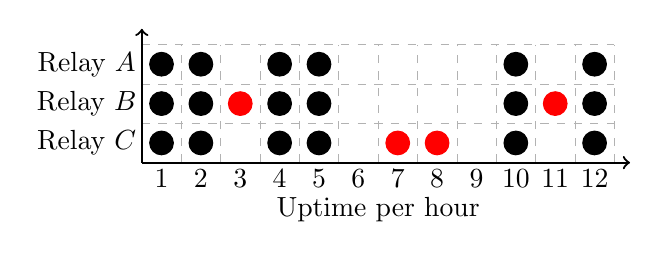
\begin{tikzpicture}
\draw[help lines, color=gray!60, dashed, step=0.5] (0,0) grid (6,1.5);
\draw[->,thick] (0,0)--(6.2,0);
\draw[->,thick] (0,0)--(0,1.7);

% Y labels.
\node at (-0.7,1.25) {Relay $A$};
\node at (-0.7,0.75) {Relay $B$};
\node at (-0.7,0.25) {Relay $C$};

% X labels.
\node at (0.25, -0.2) {1};
\node at (0.75, -0.2) {2};
\node at (1.25, -0.2) {3};
\node at (1.75, -0.2) {4};
\node at (2.25, -0.2) {5};
\node at (2.75, -0.2) {6};
\node at (3.25, -0.2) {7};
\node at (3.75, -0.2) {8};
\node at (4.25, -0.2) {9};
\node at (4.75, -0.2) {10};
\node at (5.25, -0.2) {11};
\node at (5.75, -0.2) {12};

\node at (3, -0.6) {Uptime per hour};

% Relay A.
\filldraw[black] (0.25,1.25) circle (0.15);
\filldraw[black] (0.75,1.25) circle (0.15);

\filldraw[black] (1.75,1.25) circle (0.15);
\filldraw[black] (2.25,1.25) circle (0.15);

\filldraw[black] (4.75,1.25) circle (0.15);

\filldraw[black] (5.75,1.25) circle (0.15);

% Relay B.
\filldraw[black] (0.25,0.75) circle (0.15);
\filldraw[black] (0.75,0.75) circle (0.15);
\filldraw[red]   (1.25,0.75) circle (0.15);
\filldraw[black] (1.75,0.75) circle (0.15);
\filldraw[black] (2.25,0.75) circle (0.15);

\filldraw[black] (4.75,0.75) circle (0.15);
\filldraw[red]   (5.25,0.75) circle (0.15);
\filldraw[black] (5.75,0.75) circle (0.15);

% Relay C.
\filldraw[black] (0.25,0.25) circle (0.15);
\filldraw[black] (0.75,0.25) circle (0.15);

\filldraw[black] (1.75,0.25) circle (0.15);
\filldraw[black] (2.25,0.25) circle (0.15);

\filldraw[red]   (3.25,0.25) circle (0.15);
\filldraw[red]   (3.75,0.25) circle (0.15);

\filldraw[black] (4.75,0.25) circle (0.15);

\filldraw[black] (5.75,0.25) circle (0.15);
\end{tikzpicture}

\caption{Uptime pattern of three relays.  Intuitively, relay $B$ is more
similar to relay $A$ than is relay $C$, but the Hamming distance is two for
both patterns.}
\label{fig:uptime-pattern}
\end{figure}

\begin{algorithm}[t]
\caption{Our algorithm to quantify the similarity between the uptime pattern
of two relays $A$ and $B$.}
\label{alg:uptime}
\begin{algorithmic}[1]
\Function{Distance}{$A, B$}
    \State $dist \gets 0$
    \State $amp \gets 0$

    \For{$t$ \textbf{in} $hours$}
        \If{$A_{t} \ne B_{t}$}
            \If{$amp < 1$}
                \State $amp \gets amp + 0.1$
            \EndIf
        \State $dist \gets dist + amp$
        \Else
            \State $amp \gets 0$
        \EndIf
    \EndFor
    \State \textbf{return} $dist / \lvert hours \rvert$
\EndFunction
\end{algorithmic}
\end{algorithm}

We employ Algorithm~\ref{alg:uptime} in a visualization that sybilhunter can
generate for a given set of consensuses.  The visualization is a bitmap whose
rows denote hours, and whose columns denote relays.  Every pixel in the image
represents the uptime status of a given relay.  If the pixel is black, the relay
is online, and if it is white, it is offline.  Note that this type of
visualization was first proposed by Fifield on the Tor bug
tracker~\cite{Fifield2014a}.  Similar to Fifield, we sort columns to group
similar uptime patterns together.  Our first sorting criteria is the amount of
hours a relay was online, and our second criteria is the median value of the
online sequence.  Figure~\ref{fig:uptime-matrix} gives an example, illustrating
the uptime patterns for relays in September 2011.  As columns increase, so does
the uptime of relays, until they are almost always online.  Sybils with similar
uptimes manifest as solid ``blacks'' in this type of visualization.  Refer to
Section~\ref{sec:fingerprint-anomalies} for examples.

\begin{figure}[t]
	\centering
	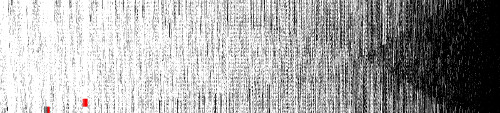
\includegraphics[width=0.48\textwidth]{diagrams/2011-09-uptimes-truncated.jpg}
	\caption{The uptime matrix for a subset of all Tor relays in September 2011.
		Every row in the image represents one consensus, and every column
		represents one relay.  As a result, every pixel denotes the uptime
		status of a given relay at a given hour.  Black pixels mean ``online,''
		white pixels mean ``offline.''  Green rows denote missing consensuses
		and red blocks denote possible Sybil groups.}
	\label{fig:uptime-matrix}
\end{figure}

Once the columns are sorted, we run our algorithm to determine the distance
between two subsequent uptime sequences.  If the distance is under our
threshold, we mark both uptime sequences as red, to make them easy to find in
manual analysis.

\subsection{Fingerprint analysis}
\label{sec:fingerprint-analysis}
The information a Tor client needs to connect to a hidden service is saved in
a distributed hash table (DHT) that consists of a subset of all Tor relays, the
hidden service directories (HSDirs).  A daily-changing set of six HSDirs are
responsible for a given hidden service.  Tor clients ask these HSDirs for
information about the hidden service they want to connect to.

A HSDir becomes responsible for a hidden service when its fingerprint
is closest to the descriptor ID that is derived from the hidden service's public
key, a time stamp, and additional information.
% https://gitweb.torproject.org/torspec.git/tree/rend-spec.txt:231
% descriptor-id = H(permanent-id | H(time-period | descriptor-cookie | replica))
Note that the DHT and all its HSDirs is known and it is also possible to
calculate which index in the fingerprint ring will be used by a hidden service
at a future point in time~\cite{Biryukov2013a}.  Attackers can exploit this
knowledge by generating identity keys until their fingerprint is close to the
hidden service's index, thus becoming responsible for it.  To save resources,
an attacker can run a single, physical Tor relay and generate a new identity
periodically.

We detect relays that change their fingerprint frequently by maintaining a
lookup table that maps a relay's IP addresses to a list of all fingerprints we
have seen it use.  We order the lookup table by the relays that changed the
fingerprints the most, and output the results.

\mynote{Elaborate.}

\subsection{Nearest-neighbor search}
\label{sec:nearest-neighbor}
We frequently found ourselves in a situation where exitmap discovered a
malicious exit relay and we were trying to find similar, potentially associated
relays.  This involved extensive manual work, which we soon started to automate.
In particular, we needed an algorithm for nearest-neighbor search: given a
``seed'' relay, what are its $n$ nearest neighbors?

A naive implementation would compare the seed relay to all other relays in the
consensus, which scales linearly.  We can do better by using metric trees, which
guarantee $\mathcal{O}(\textrm{log} n)$ lookup.  Metric trees are a type of data
structure to index data in metric spaces.  Metric trees require a distance
metric in the mathematical sense, i.e., a number of conditions to be met (see
Appendix~\ref{sec:metric}), which are not always satisfied by ad-hoc metrics.
% In particular, the triangle inequality\footnote{The triangle inequality, $d(x,
% z) \le d(x, y) + d(y, z)$, states that the distance between two points is at
% least equal to a ``detour'' over a third point.} can be difficult to meet when
% working in non-Euclidean space.

\mynote{Explain more rigorously.}

We use the Levenshtein distance as distance metric.  It operates on strings and
determines the minimum amount of modifications---insert, delete, and
modify---that are necessary to turn string $s_{1}$ into $s_{2}$.  The
Levenshtein distance can handle strings of different length, and satisfies the
triangle inequality, i.e., we are free to use it in a metric tree.

As concrete metric tree implementation, we use the vantage point tree
(vp-tree)~\cite{Yianilos1993a}.  It recursively divides the given data into two
partitions; one that is close to the seed point according to a threshold,
and one that is not.  The vp-tree must first be built for the given data, and it
is then ready to perform nearest neighbor searches.

\mynote{Talk about how long it takes to build the tree.}

In our implementation, building a vp-tree for 6,235 relays takes approximately
10 seconds.\footnote{Again, measured on an Intel Core i7 2.9 GHz CPU.}
Subsequent nearest-neighbor lookups finish almost instantly.

\mynote{Still need to compare this to naive $n^{2}$ search.}

\subsection{Blocking Sybils}
Once we isolated a Sybil group, and concluded that it appears to be harmful, we
reported it to The Tor Project.  There are currently two ways for directory
authorities to block relays, controlled by the options \texttt{AuthDirReject}
and \texttt{AuthDirInvalid}.  The former removes a relay from the consensus.
The latter takes away a relay's \texttt{Valid} flag.  While the relay is still
listed in the consensus, clients will not consider it for path selection.

The majority of directory authorities, i.e., four out of eight, must agree on
either \texttt{AuthDirReject} or \texttt{AuthDirInvalid} be set for a relay.
Only then will the block become active.  This mechanism is meant to distribute
the power of removing relays into the hands of a diverse set of people.  We
elaborate on our experience with this process in Section~\ref{sec:operational}.

\subsection{Meaningful results}
Systems that employ complex and opaque analysis techniques to expose security
incidents frequently suffer from what Sommer and Paxson call the \emph{semantic
gap}~\cite[\S III.C]{Sommer2010a}, i.e., a system's output is difficult to act
upon as its meaning is unclear.  Our tools automate the detection of Sybils,
but the process of blocking them involves human interaction, which is why we
took special care to consider the semantic gap.

We avoid the use of opaque classification methods as their output (often a
distance in high-dimensional vector space) is difficult to interpret.  Instead,
we rely on straightforward metrics such as the Levenshtein distance.
Figure~\ref{fig:visualization} further illustrates a visualization that we
developed for exploratory analysis, which is meant to complement automated
analysis.  The graph shows the similarities (edges) between four Tor relays
(vertices).

\begin{figure}[t]
	\centering
	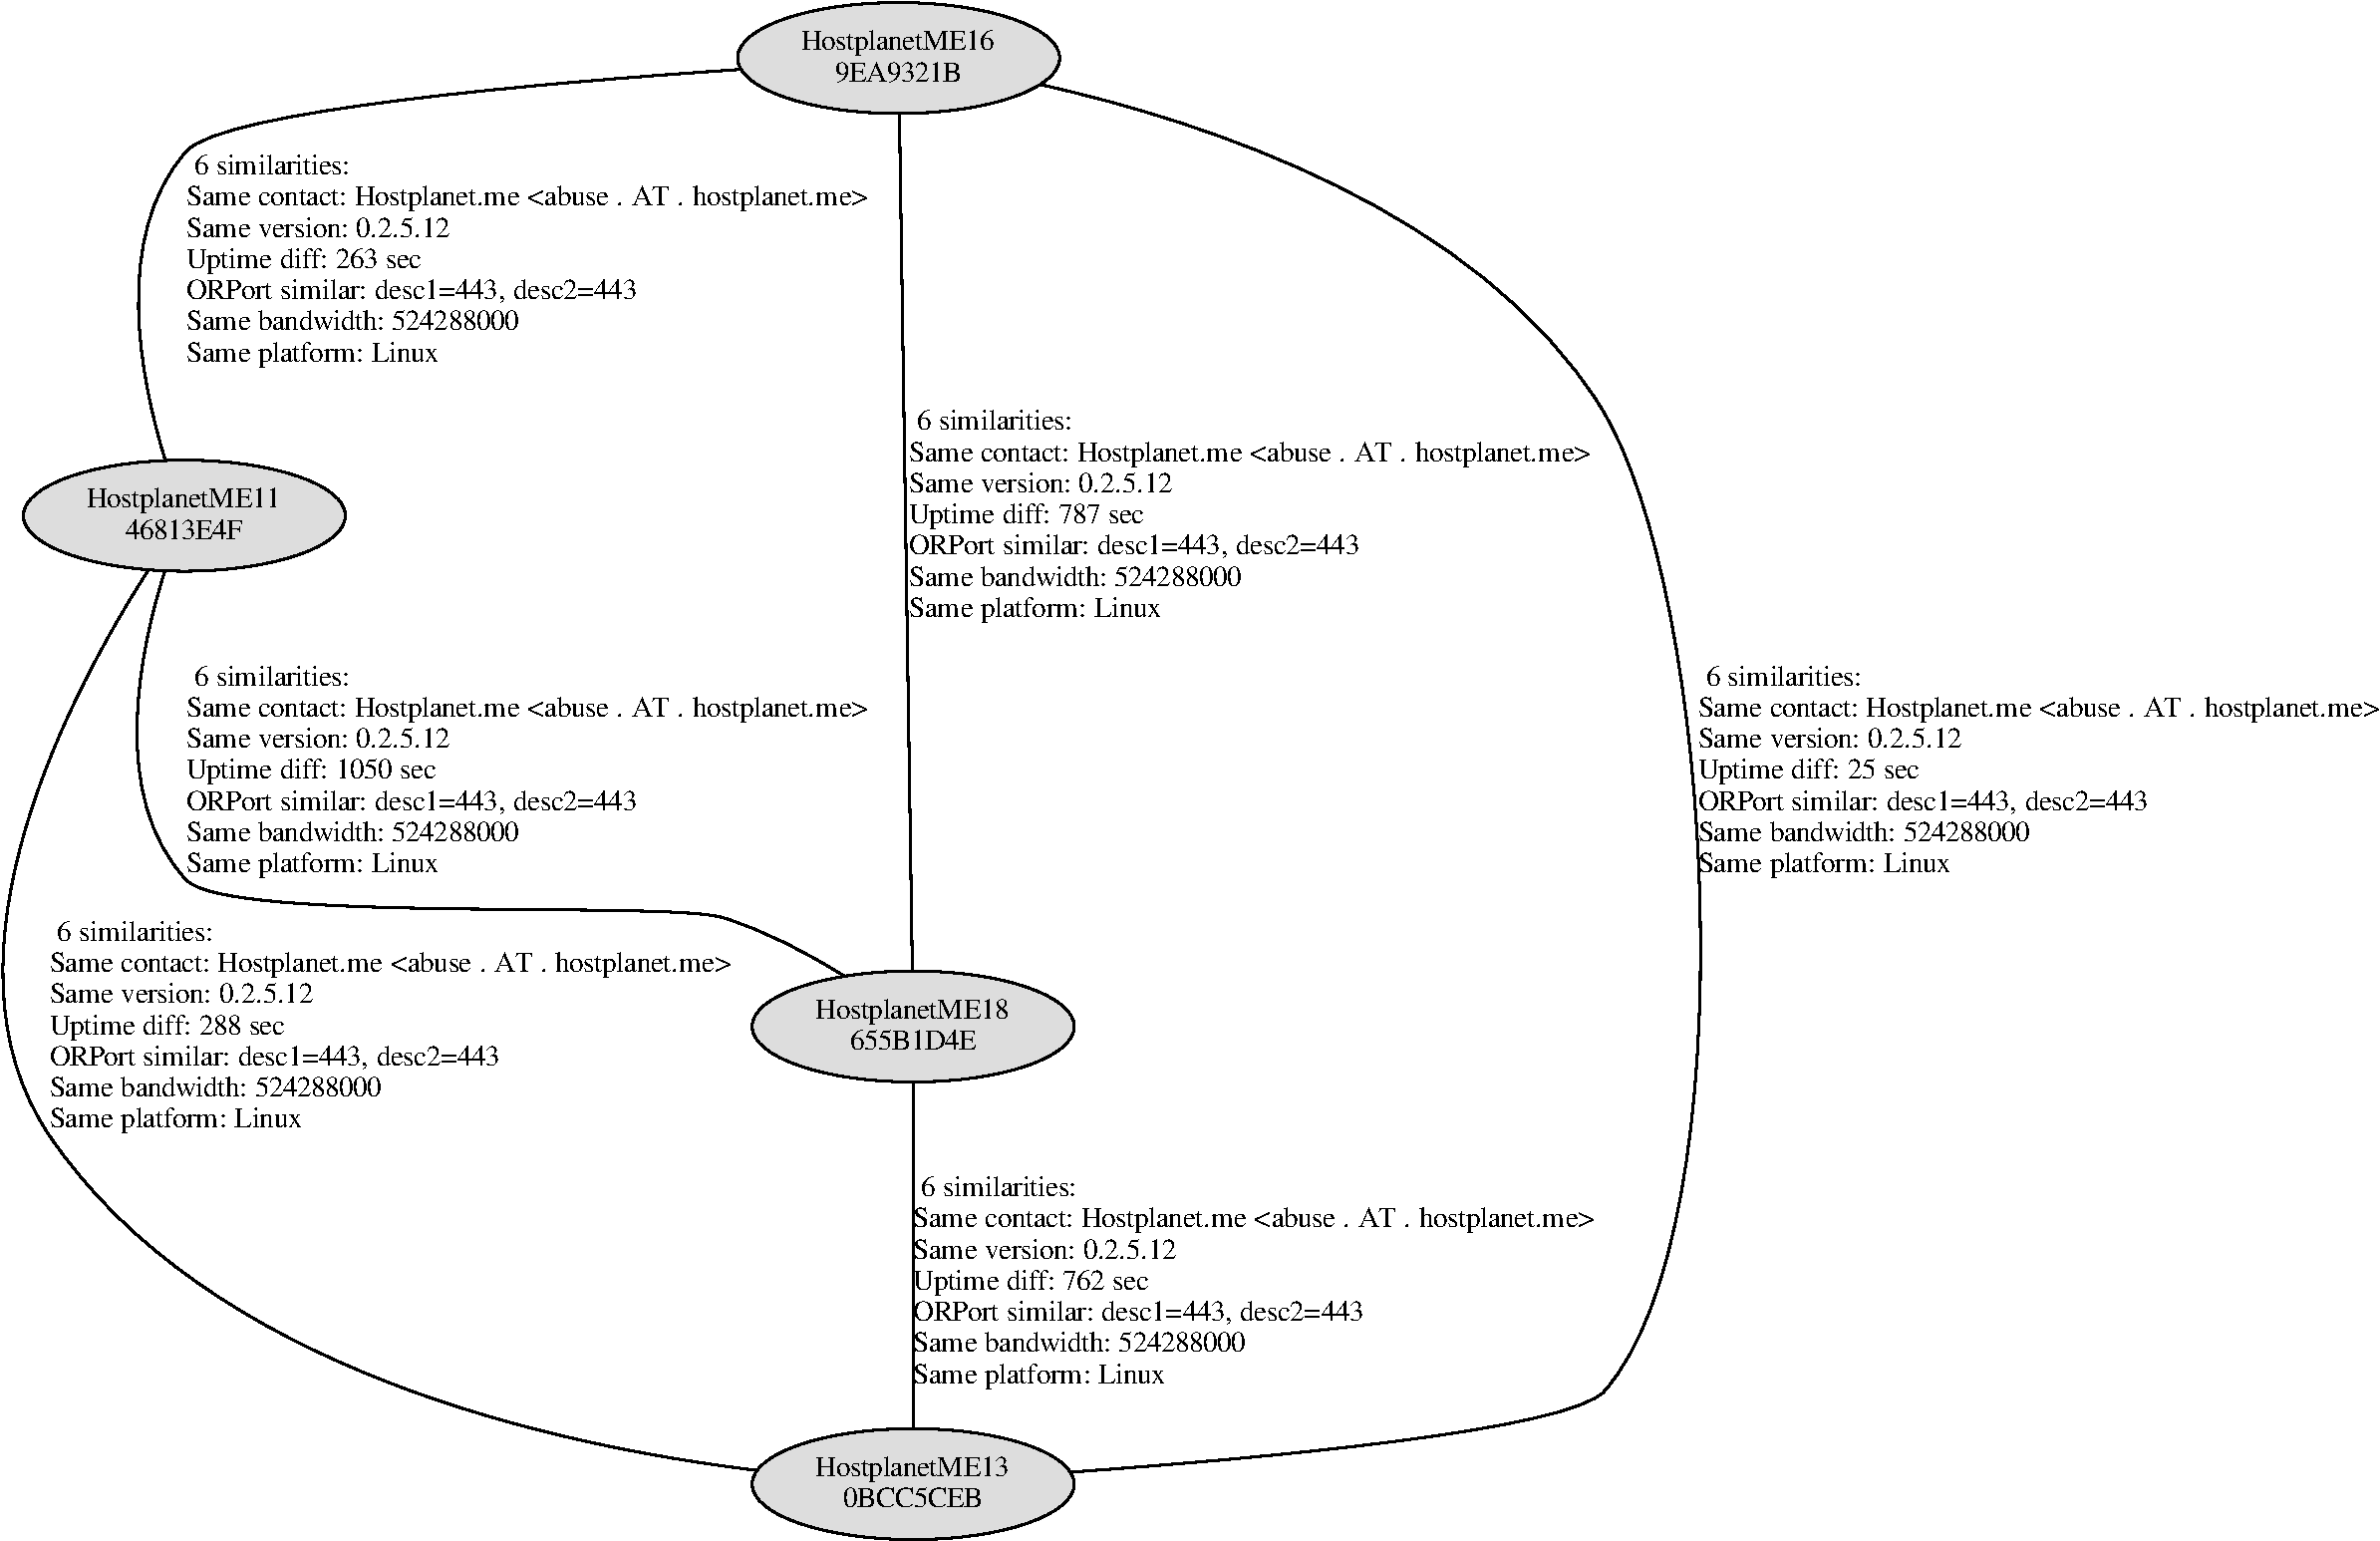
\includegraphics[width=0.42\textwidth]{diagrams/visualization.pdf}
    \caption{Visualization of a Sybil cluster.  Vertices represent Tor relays
    and edges show the similarities between them.}
	\label{fig:visualization}
\end{figure}
